% Options for packages loaded elsewhere
\PassOptionsToPackage{unicode}{hyperref}
\PassOptionsToPackage{hyphens}{url}
%
\documentclass[
]{article}
\usepackage{amsmath,amssymb}
\usepackage{lmodern}
\usepackage{iftex}
\ifPDFTeX
  \usepackage[T1]{fontenc}
  \usepackage[utf8]{inputenc}
  \usepackage{textcomp} % provide euro and other symbols
\else % if luatex or xetex
  \usepackage{unicode-math}
  \defaultfontfeatures{Scale=MatchLowercase}
  \defaultfontfeatures[\rmfamily]{Ligatures=TeX,Scale=1}
\fi
% Use upquote if available, for straight quotes in verbatim environments
\IfFileExists{upquote.sty}{\usepackage{upquote}}{}
\IfFileExists{microtype.sty}{% use microtype if available
  \usepackage[]{microtype}
  \UseMicrotypeSet[protrusion]{basicmath} % disable protrusion for tt fonts
}{}
\makeatletter
\@ifundefined{KOMAClassName}{% if non-KOMA class
  \IfFileExists{parskip.sty}{%
    \usepackage{parskip}
  }{% else
    \setlength{\parindent}{0pt}
    \setlength{\parskip}{6pt plus 2pt minus 1pt}}
}{% if KOMA class
  \KOMAoptions{parskip=half}}
\makeatother
\usepackage{xcolor}
\IfFileExists{xurl.sty}{\usepackage{xurl}}{} % add URL line breaks if available
\IfFileExists{bookmark.sty}{\usepackage{bookmark}}{\usepackage{hyperref}}
\hypersetup{
  pdftitle={P2 S6 Presentación},
  pdfauthor={Grupo 6},
  hidelinks,
  pdfcreator={LaTeX via pandoc}}
\urlstyle{same} % disable monospaced font for URLs
\usepackage[margin=1in]{geometry}
\usepackage{color}
\usepackage{fancyvrb}
\newcommand{\VerbBar}{|}
\newcommand{\VERB}{\Verb[commandchars=\\\{\}]}
\DefineVerbatimEnvironment{Highlighting}{Verbatim}{commandchars=\\\{\}}
% Add ',fontsize=\small' for more characters per line
\usepackage{framed}
\definecolor{shadecolor}{RGB}{248,248,248}
\newenvironment{Shaded}{\begin{snugshade}}{\end{snugshade}}
\newcommand{\AlertTok}[1]{\textcolor[rgb]{0.94,0.16,0.16}{#1}}
\newcommand{\AnnotationTok}[1]{\textcolor[rgb]{0.56,0.35,0.01}{\textbf{\textit{#1}}}}
\newcommand{\AttributeTok}[1]{\textcolor[rgb]{0.77,0.63,0.00}{#1}}
\newcommand{\BaseNTok}[1]{\textcolor[rgb]{0.00,0.00,0.81}{#1}}
\newcommand{\BuiltInTok}[1]{#1}
\newcommand{\CharTok}[1]{\textcolor[rgb]{0.31,0.60,0.02}{#1}}
\newcommand{\CommentTok}[1]{\textcolor[rgb]{0.56,0.35,0.01}{\textit{#1}}}
\newcommand{\CommentVarTok}[1]{\textcolor[rgb]{0.56,0.35,0.01}{\textbf{\textit{#1}}}}
\newcommand{\ConstantTok}[1]{\textcolor[rgb]{0.00,0.00,0.00}{#1}}
\newcommand{\ControlFlowTok}[1]{\textcolor[rgb]{0.13,0.29,0.53}{\textbf{#1}}}
\newcommand{\DataTypeTok}[1]{\textcolor[rgb]{0.13,0.29,0.53}{#1}}
\newcommand{\DecValTok}[1]{\textcolor[rgb]{0.00,0.00,0.81}{#1}}
\newcommand{\DocumentationTok}[1]{\textcolor[rgb]{0.56,0.35,0.01}{\textbf{\textit{#1}}}}
\newcommand{\ErrorTok}[1]{\textcolor[rgb]{0.64,0.00,0.00}{\textbf{#1}}}
\newcommand{\ExtensionTok}[1]{#1}
\newcommand{\FloatTok}[1]{\textcolor[rgb]{0.00,0.00,0.81}{#1}}
\newcommand{\FunctionTok}[1]{\textcolor[rgb]{0.00,0.00,0.00}{#1}}
\newcommand{\ImportTok}[1]{#1}
\newcommand{\InformationTok}[1]{\textcolor[rgb]{0.56,0.35,0.01}{\textbf{\textit{#1}}}}
\newcommand{\KeywordTok}[1]{\textcolor[rgb]{0.13,0.29,0.53}{\textbf{#1}}}
\newcommand{\NormalTok}[1]{#1}
\newcommand{\OperatorTok}[1]{\textcolor[rgb]{0.81,0.36,0.00}{\textbf{#1}}}
\newcommand{\OtherTok}[1]{\textcolor[rgb]{0.56,0.35,0.01}{#1}}
\newcommand{\PreprocessorTok}[1]{\textcolor[rgb]{0.56,0.35,0.01}{\textit{#1}}}
\newcommand{\RegionMarkerTok}[1]{#1}
\newcommand{\SpecialCharTok}[1]{\textcolor[rgb]{0.00,0.00,0.00}{#1}}
\newcommand{\SpecialStringTok}[1]{\textcolor[rgb]{0.31,0.60,0.02}{#1}}
\newcommand{\StringTok}[1]{\textcolor[rgb]{0.31,0.60,0.02}{#1}}
\newcommand{\VariableTok}[1]{\textcolor[rgb]{0.00,0.00,0.00}{#1}}
\newcommand{\VerbatimStringTok}[1]{\textcolor[rgb]{0.31,0.60,0.02}{#1}}
\newcommand{\WarningTok}[1]{\textcolor[rgb]{0.56,0.35,0.01}{\textbf{\textit{#1}}}}
\usepackage{longtable,booktabs,array}
\usepackage{calc} % for calculating minipage widths
% Correct order of tables after \paragraph or \subparagraph
\usepackage{etoolbox}
\makeatletter
\patchcmd\longtable{\par}{\if@noskipsec\mbox{}\fi\par}{}{}
\makeatother
% Allow footnotes in longtable head/foot
\IfFileExists{footnotehyper.sty}{\usepackage{footnotehyper}}{\usepackage{footnote}}
\makesavenoteenv{longtable}
\usepackage{graphicx}
\makeatletter
\def\maxwidth{\ifdim\Gin@nat@width>\linewidth\linewidth\else\Gin@nat@width\fi}
\def\maxheight{\ifdim\Gin@nat@height>\textheight\textheight\else\Gin@nat@height\fi}
\makeatother
% Scale images if necessary, so that they will not overflow the page
% margins by default, and it is still possible to overwrite the defaults
% using explicit options in \includegraphics[width, height, ...]{}
\setkeys{Gin}{width=\maxwidth,height=\maxheight,keepaspectratio}
% Set default figure placement to htbp
\makeatletter
\def\fps@figure{htbp}
\makeatother
\setlength{\emergencystretch}{3em} % prevent overfull lines
\providecommand{\tightlist}{%
  \setlength{\itemsep}{0pt}\setlength{\parskip}{0pt}}
\setcounter{secnumdepth}{-\maxdimen} % remove section numbering
\ifLuaTeX
  \usepackage{selnolig}  % disable illegal ligatures
\fi

\title{P2 S6 Presentación}
\author{Grupo 6}
\date{24, Junio, 2022}

\begin{document}
\maketitle

{
\setcounter{tocdepth}{2}
\tableofcontents
}
\hypertarget{integrantes}{%
\section{\texorpdfstring{\textbf{Integrantes}}{Integrantes}}\label{integrantes}}

\begin{longtable}[]{@{}
  >{\raggedright\arraybackslash}p{(\columnwidth - 4\tabcolsep) * \real{0.5119}}
  >{\raggedright\arraybackslash}p{(\columnwidth - 4\tabcolsep) * \real{0.1548}}
  >{\raggedright\arraybackslash}p{(\columnwidth - 4\tabcolsep) * \real{0.3333}}@{}}
\toprule
\endhead
\textbf{Apellidos y Nombres} & \textbf{Código} & \textbf{Carrera} \\
Santillan Socla, Helen Jadhira (Líder) & 202120530 & Ingeniería
Industrial \\
Raza Estrada, Gilver Alexis & 202020129 & Ciencia de la Computación \\
Farfán Gonzales, Gabriel Mauricio & 201910503 & Ingeniería Química \\
Colque Ale, Walther Jesús & 202120168 & Ingeniería Industrial \\
Choqque Mejia, Fernando Adriano & 202020038 & Ciencia de la
Computación \\
\bottomrule
\end{longtable}

\hypertarget{introducciuxf3n}{%
\section{\texorpdfstring{\textbf{Introducción}}{Introducción}}\label{introducciuxf3n}}

\hypertarget{relevancia}{%
\subsection{\texorpdfstring{\textbf{Relevancia}}{Relevancia}}\label{relevancia}}

El 15 de marzo del 2020 a causa del confinamiento hizo que muchas
actividades se realizaran de manera virtual, y la compra de productos
tecnológicos no se hicieron de esperar. Debido a que muchas personas
necesitaban un aparato tecnológico para su uso, muchas de estas
decidieron recurrir a sus compras, pero de manera online, evitando de
esa manera una manera de contagio.

Este nuevo método de comprar de forma online fue progresivo. Asimismo,
la tecnología estuvo de nuestro lado y facilitó a su vez la adaptación;
ya que, no solo podíamos visualizar los productos desde casa, sino que
también nos permitía comparar precios para luego hacer la elección más
favorable, sin necesidad de salir de casa.

En este proyecto, vamos a evaluar el grado de adaptacion, es decir, que
tanto se han adaptado las personas de los distritos de la ciudad de Lima
- Peru hacia estasc compras de productos tecnologicos de manera online.
Estos resultados también nos servirá como indicador de la confiabilidad
hacia la modalidad de compra online.

Para ello analizaremos los datos obtenidos por personas de los distritos
de la ciudad de Lima, mediante una encuesta de Google Forms. Luego,
realizaremos la respectiva limpieza de datos, un análisis descriptivo y
un análisis probabilistico, de tal manera que podamos mencionar que
distrito se ha adaptado con la modalidad de compra online de productos
tecnologico.

\textbf{Variables Cualitativas:} Sexo, Distrito, Empresa, Producto y
Marca.

\textbf{Variables Cuantitativas:} Precio, Edad, Tiempo de garantía del
producto (Meses), Año en el que adquirió el producto y Que tanto
calificas del 1 al 10 la llegada del producto a tu domicilio.

\begin{Shaded}
\begin{Highlighting}[]
\CommentTok{\# Instalación y apertura de librerías}

\ControlFlowTok{if}\NormalTok{(}\SpecialCharTok{!}\FunctionTok{require}\NormalTok{(readr))\{}\FunctionTok{install.packages}\NormalTok{(}\StringTok{"readr"}\NormalTok{)\}}
\ControlFlowTok{if}\NormalTok{(}\SpecialCharTok{!}\FunctionTok{require}\NormalTok{(dplyr))\{}\FunctionTok{install.packages}\NormalTok{(}\StringTok{"dplyr"}\NormalTok{)\}}
\ControlFlowTok{if}\NormalTok{(}\SpecialCharTok{!}\FunctionTok{require}\NormalTok{(ggplot2))\{}\FunctionTok{install.packages}\NormalTok{(}\StringTok{"ggplot2"}\NormalTok{)\}}
\ControlFlowTok{if}\NormalTok{(}\SpecialCharTok{!}\FunctionTok{require}\NormalTok{(ggthemes))\{}\FunctionTok{install.packages}\NormalTok{(}\StringTok{"ggthemes"}\NormalTok{)\}}

\FunctionTok{library}\NormalTok{(readr)}
\FunctionTok{library}\NormalTok{(dplyr)}
\FunctionTok{library}\NormalTok{(ggplot2)}
\FunctionTok{library}\NormalTok{(ggthemes)}
\end{Highlighting}
\end{Shaded}

\hypertarget{planificaciuxf3n}{%
\subsection{\texorpdfstring{\textbf{Planificación}}{Planificación}}\label{planificaciuxf3n}}

En base a la planificación, se tiene que cada uno hemos invertido entre
3 y 4 horas al proyecto, de tal manera que podemos observar que han sido
2 personas las que se han encargado de la parte de codificación y el
resto se encargó de la parte del estudio de la base de datos. De acuerdo
a la disponibilidad de todo el grupo, coordinamos para realizar una
reunión general para poder ver el avance total del proyecto

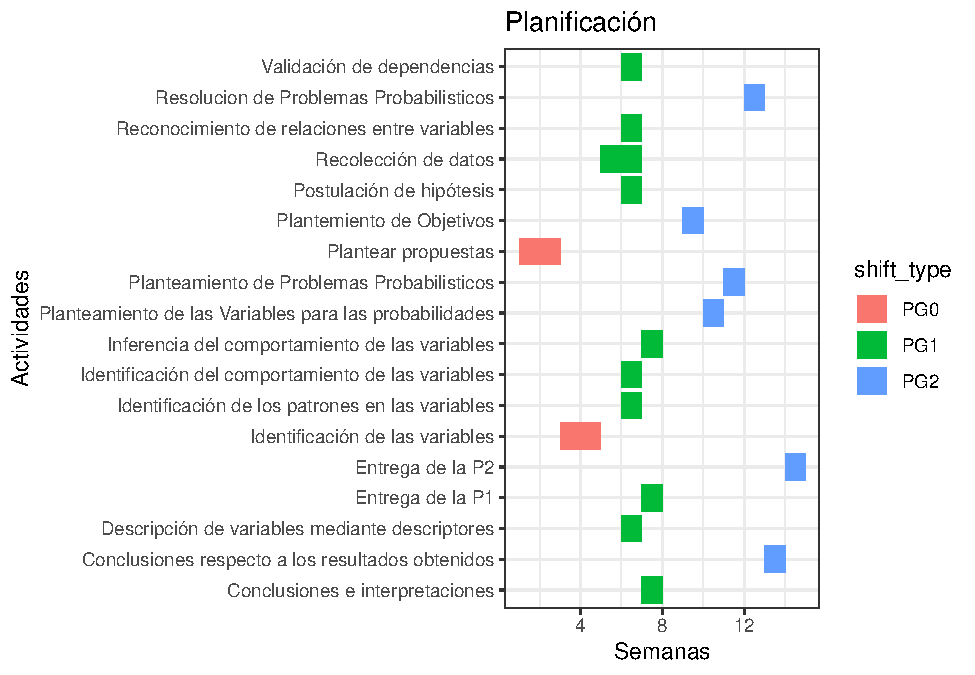
\includegraphics{S6_Informe_files/figure-latex/unnamed-chunk-2-1.pdf}

\hypertarget{datos}{%
\section{\texorpdfstring{\textbf{Datos}}{Datos}}\label{datos}}

\hypertarget{recolecciuxf3n-de-datos}{%
\subsection{\texorpdfstring{\textbf{Recolección de
datos}}{Recolección de datos}}\label{recolecciuxf3n-de-datos}}

La técnica que se utilizó con la finalidad de recolectar datos para el
estudio fue la encuesta mediante Google Forms, la cual estuvo compuesto
por 12 preguntas donde 10 de ellas eran de alta relevancia para lo
requerido en nuestro proyecto. Nuestro público dirigido no solo fue a
estudiantes de UTEC sino también a individuos en general que hayan
realizado una compra durante los 3 años establecidos. El uso de las
redes sociales (WhatsApp y otros) fue necesario para alcanzar los 200
datos requeridos y para generar el interés en la unidad muestral fue
necesario realizar un sorteo de 50 nuevos soles.


\includegraphics{encuesta.jpg}

\hypertarget{poblaciuxf3n-muestra-y-muestreo}{%
\subsection{\texorpdfstring{\textbf{Población, muestra y
muestreo}}{Población, muestra y muestreo}}\label{poblaciuxf3n-muestra-y-muestreo}}

Población, muestra y muestreo: La población escogida son las personas de
Lima - Perú y la unidad muestral es aquella persona que vive en
cualquier distrito de la población. El tipo de muestreo utilizado es un
muestreo por conveniencia. Finalmente luego de hacer la limpieza de
datos nuestro tamaño de la muestra es de 172.

\hypertarget{variables}{%
\subsection{\texorpdfstring{\textbf{Variables}}{Variables}}\label{variables}}

En primera instancia tenemos 13 variables de las cuáles 2 son
irrelevantes para el estudio Estadístico ya que una de ellas ( Marca
Temporal) es generada por Google Forms. Asimismo, la variable Correo
sirve básicamente para poder contactar a la persona ganadora del sorteo.
Finalmente trabajaremos con 11 variables y son las siguientes:

\begin{itemize}
\item
  Nombre: tipo categórica nominal, la restricción es que sea un nombre
  registrado en el RENIEC. ✔
\item
  Sexo: tipo categórica nominal, la restricción es que pertenezca al
  sexo Masculino o Femenino. ✔
\item
  Distrito: tipo categórica nominal, la restricción es que el distrito
  pertenezca a uno de los distritos en Lima-Perú. ✔
\item
  Edad: tipo numérica discreta, la restricción es que sea un entero
  positivo. ✔
\item
  Empresa: tipo categórica nominal, no tiene restricción. ✔
\item
  Producto: tipo categórica nominal, la restricción es que el producto
  sea un aparato tecnológico comprado de manera online. ✔
\item
  Marca: tipo categórica nomianal, la restricción es que la marca esté
  patentada por INDECOPI. ✔
\item
  Precio: tipo numérica continua, la restricción es que sea un número
  racional positivo. ✔
\item
  Garantia: tipo numérica discreta, la restricción es que sea un entero
  no negativo. ✔
\item
  Año: tipo categórica ordinal, la restricción es que el año en que se
  realizó la compra sea de 2020 al 2022, ya que es el periodo de
  pandemia. ✔
\item
  Calificacion: tipo numérica discreta, la restricción es que sea un
  entero no negativo entre 1 y 10. ✔
\end{itemize}

\hypertarget{limpieza}{%
\subsection{\texorpdfstring{\textbf{Limpieza}}{Limpieza}}\label{limpieza}}

\begin{verbatim}
## Warning: NAs introducidos por coerción
\end{verbatim}

\begin{itemize}
\item
  \textbf{Sexo:}

  \begin{itemize}
  \tightlist
  \item
    convertir todos los valores a F, M o NA
  \end{itemize}
\item
  \textbf{Distrito:}

  \begin{itemize}
  \item
    convertir las diferentes formas de escribir un distrito a solo una
    (ej: VES, ves, v.e.s a V.E.S)
  \item
    Solo distritos de Lima, los no pertenecientes se eliminan de la base
    de datos
  \end{itemize}
\item
  \textbf{Empresa, Producto y Marca:}

  \begin{itemize}
  \item
    Solo productos tecnológicos, los no pertenecientes se eliminan de la
    base de datos
  \item
    Relación coherente entre Empresa - Producto - Marca
  \end{itemize}
\item
  \textbf{Precio:}

  \begin{itemize}
  \tightlist
  \item
    Valores como ``40 dólares, 20 soles, etc'' convertidos a solo valor
    en soles
  \end{itemize}
\end{itemize}

\hypertarget{anuxe1lisis-descriptivo}{%
\section{\texorpdfstring{\textbf{Análisis
Descriptivo}}{Análisis Descriptivo}}\label{anuxe1lisis-descriptivo}}

\hypertarget{descriptores-gruxe1ficos}{%
\subsection{\texorpdfstring{\textbf{Descriptores
gráficos}}{Descriptores gráficos}}\label{descriptores-gruxe1ficos}}

\hypertarget{distritos-con-mayores-compras}{%
\subsubsection{\texorpdfstring{\textbf{Distritos con mayores
compras}}{Distritos con mayores compras}}\label{distritos-con-mayores-compras}}

Hemos seleccionado los distritos con compras online mayores o igual a
10. En primer lugar tenemos al distrito de S.J.L con 21 compras, en
segundo lugar tenemos al distrito de Los Olivos con 17 compras, y en el
tercer lugar tenemos a los distritos S.M.P y Surco con 15 compras.
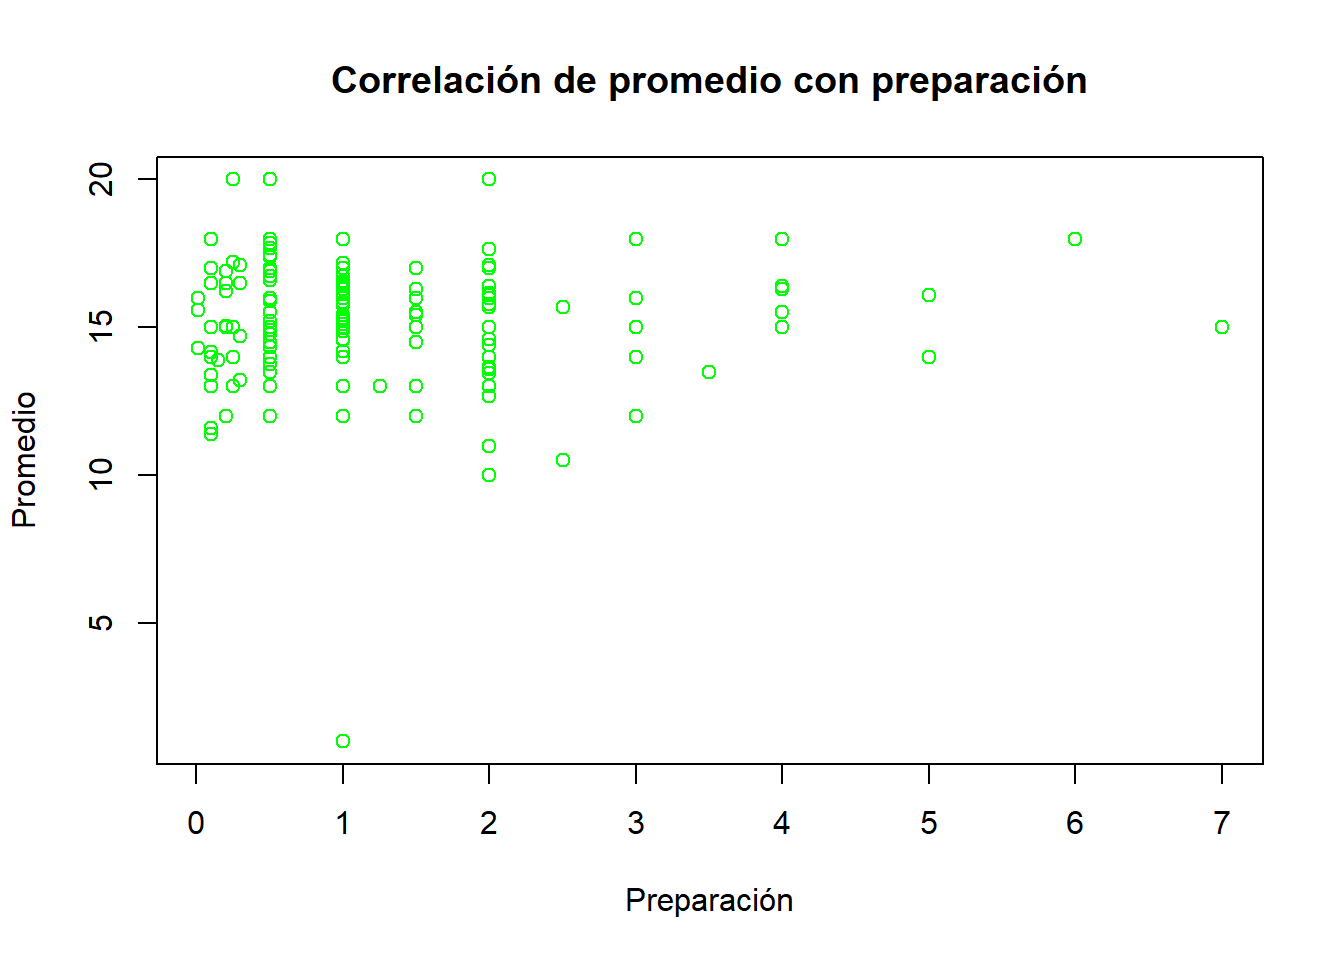
\includegraphics{S6_Informe_files/figure-latex/unnamed-chunk-11-1.pdf}
\#\#\# \textbf{Número de Compras por Año}

También podemos observar que el año en el cual se han realizado la mayor
cantidad de compras es en el 2021 (96 compras).
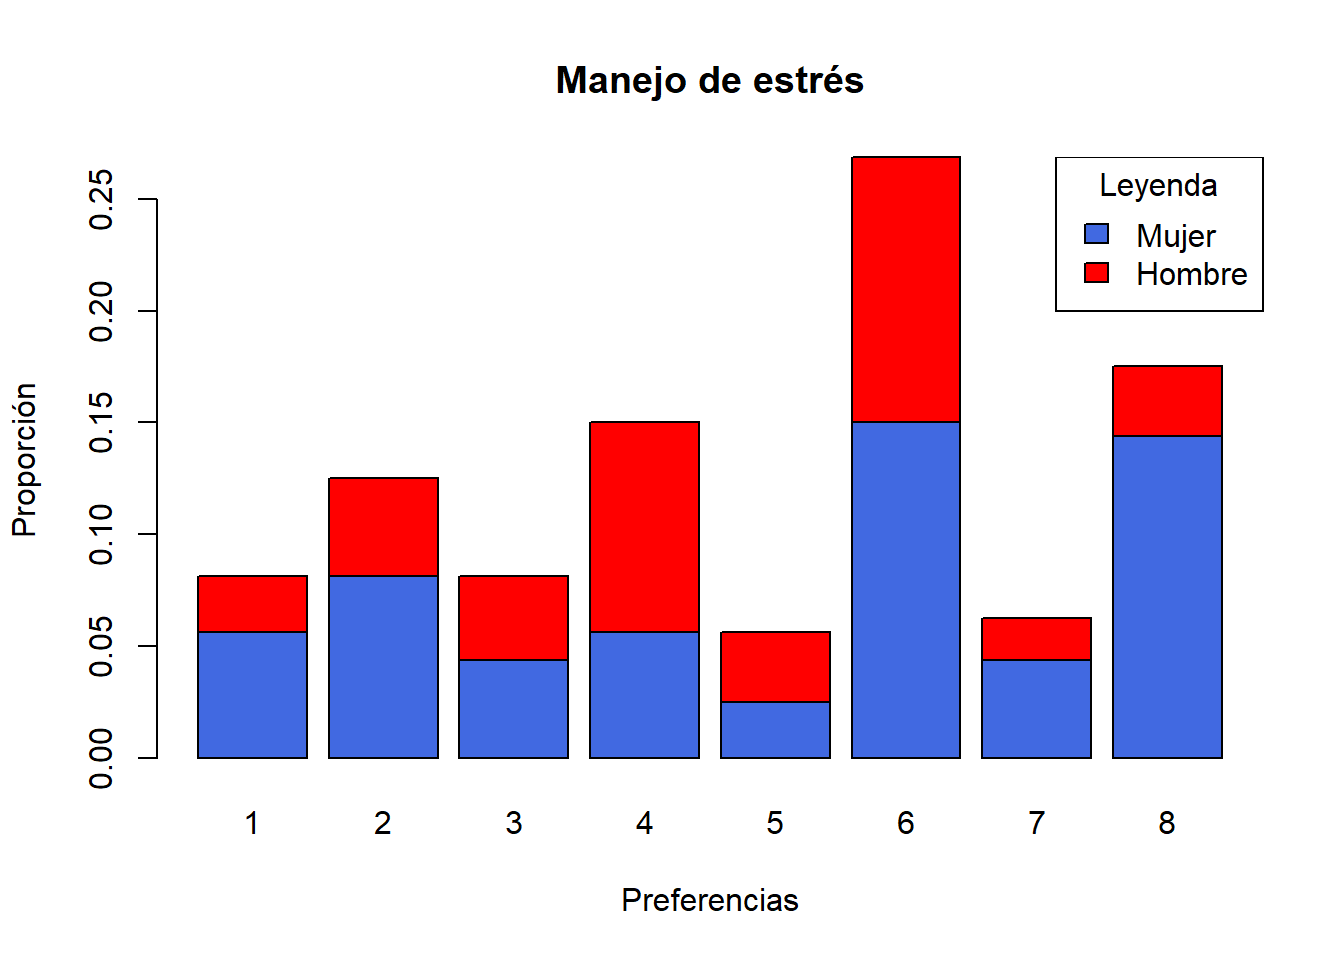
\includegraphics{S6_Informe_files/figure-latex/unnamed-chunk-12-1.pdf}

\hypertarget{garantuxeda}{%
\subsubsection{\texorpdfstring{\textbf{Garantía}}{Garantía}}\label{garantuxeda}}

Esta gráfica nos indica las diferentes garantías ofrecidas para cada
producto. Se observa que la Garantía está concentrada entre 6 y 12
meses. Sin embargo, existen 3 datos atípicos, que indican que las
personas que compraron de manera online un producto tecnológico optaron
por una garantía mucho mayor a la promedio.

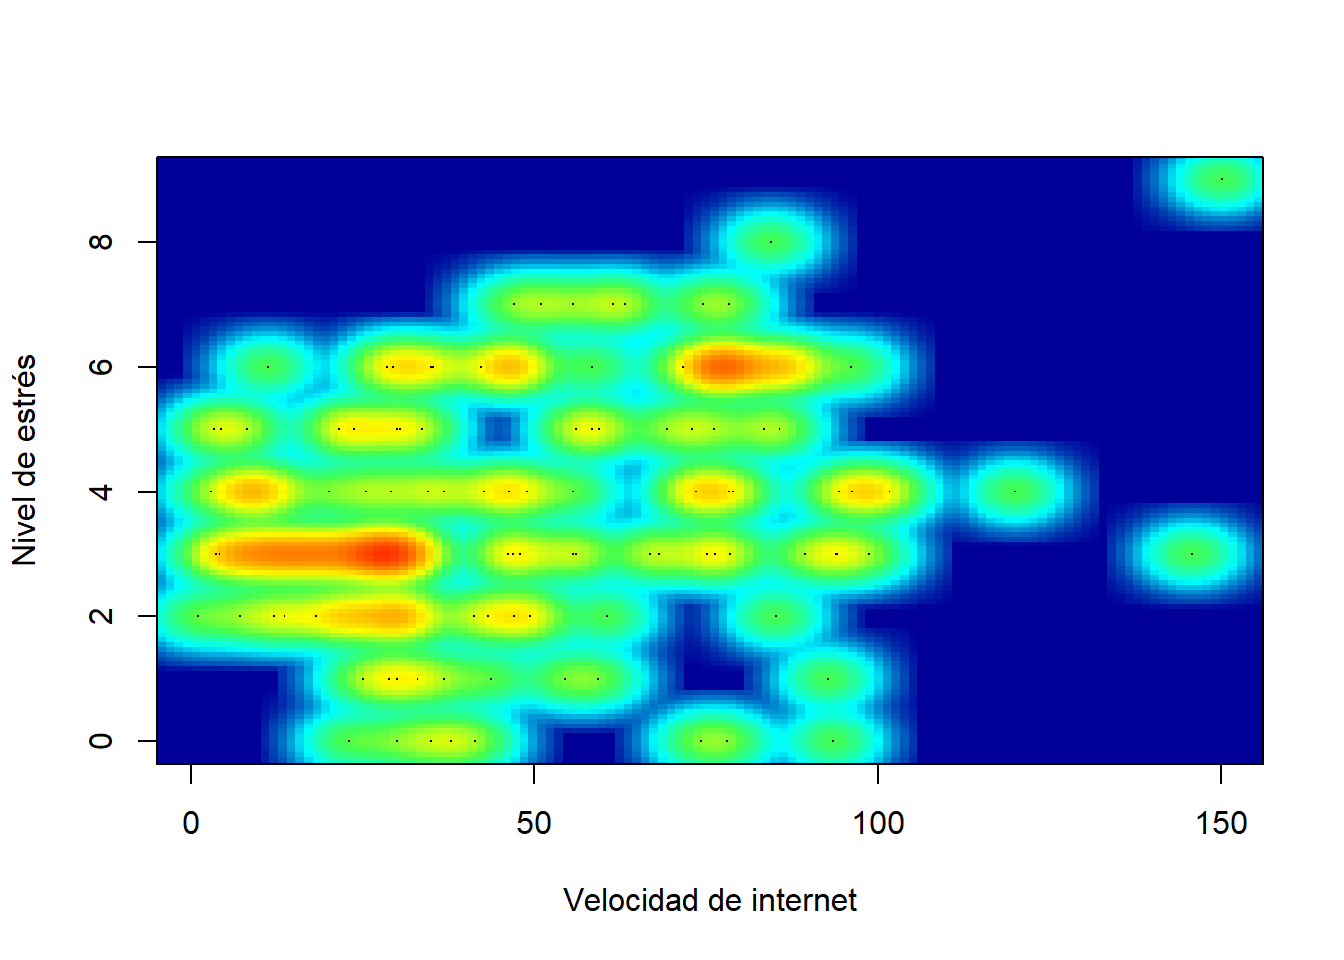
\includegraphics{S6_Informe_files/figure-latex/unnamed-chunk-13-1.pdf}

\hypertarget{descriptores-numuxe9ricos}{%
\subsection{\texorpdfstring{\textbf{Descriptores
numéricos}}{Descriptores numéricos}}\label{descriptores-numuxe9ricos}}

Los productos mayormente ofrecen una garantía de 12 meses (moda)

\begin{verbatim}
## Garantia
##  0  1  2  3  5  6  8  9 12 18 24 36 48 
##  9 18  2  8  1 20  3  3 83  5 11  1  1
\end{verbatim}

El precio promedio es de S/ 1724.00 y vemos que el mínimo y máximo
precio de un producto son S/ 2.1 y S/ 9999.00 respectivamente. También,
la calificación promedio otorgada a la Empresa en donde se hizo la
compra online es de 8.36 (muestra un alto grado de conformidad con la
Empresa).

\begin{verbatim}
##        Precio  Garantía Calificación
## Min    2.1     0        1           
## Max    9999    48       10          
## Mean   1724    10.04    8.36        
## Median 1050    12       9           
## SD     1807.74 7.06     1.75        
## CV     1.05    0.7      0.21        
## IQR    2625    6        2
\end{verbatim}

\hypertarget{anuxe1lisis-probabilistico}{%
\section{\texorpdfstring{\textbf{Análisis
Probabilistico}}{Análisis Probabilistico}}\label{anuxe1lisis-probabilistico}}

\hypertarget{modelos-de-variables-discretas}{%
\subsection{\texorpdfstring{\textbf{Modelos de Variables
Discretas}}{Modelos de Variables Discretas}}\label{modelos-de-variables-discretas}}

\hypertarget{aplicaciuxf3n-del-modelo-binomial-negativo}{%
\subsubsection{\texorpdfstring{\textbf{Aplicación del Modelo Binomial
Negativo}}{Aplicación del Modelo Binomial Negativo}}\label{aplicaciuxf3n-del-modelo-binomial-negativo}}

Queremos seleccionar a los 2 ganadores del sorteo, los pondremos en una
ruleta para elegir a los ganadores. Cuán probable es de que los
ganadores del sorteo pertenezcan al distrito con mayor compras online
(S.J.L).

\begin{itemize}
\tightlist
\item
  Éxito -\textgreater{} personas que pertenezcan al Distrito con más
  compras online (SJL)
\item
  Fracaso -\textgreater{} personas que no pertenezcan al Distrito con
  más compras online (SJL)
\end{itemize}

Variable aleatoria: 𝑿=\# de sorteos realizados hasta tener k éxitos.

\begin{itemize}
\tightlist
\item
  P(éxito) : 21 (\# personas de S.JL) / 172 (\# total de personas)
\item
  k : queremos 2 ganadores del distrito de S.J.L
\end{itemize}

Definimos variablels en R:

\begin{Shaded}
\begin{Highlighting}[]
\NormalTok{X }\OtherTok{=} \DecValTok{2}
\NormalTok{k }\OtherTok{=} \DecValTok{2}
\NormalTok{total }\OtherTok{=} \DecValTok{172}
\NormalTok{CO }\OtherTok{=} \DecValTok{21}
\NormalTok{Pe }\OtherTok{=}\NormalTok{ CO}\SpecialCharTok{/}\NormalTok{total}

\FunctionTok{choose}\NormalTok{(X}\DecValTok{{-}1}\NormalTok{, k}\DecValTok{{-}1}\NormalTok{)}\SpecialCharTok{*}\NormalTok{(Pe}\SpecialCharTok{\^{}}\NormalTok{k)}\SpecialCharTok{*}\NormalTok{((}\DecValTok{1}\SpecialCharTok{{-}}\NormalTok{Pe)}\SpecialCharTok{\^{}}\NormalTok{(X}\SpecialCharTok{{-}}\NormalTok{k))}
\end{Highlighting}
\end{Shaded}

\begin{verbatim}
## [1] 0.01490671
\end{verbatim}

Con el comando ``dnbinom'':

\begin{Shaded}
\begin{Highlighting}[]
\FunctionTok{dnbinom}\NormalTok{(X}\SpecialCharTok{{-}}\NormalTok{k, k, Pe)}
\end{Highlighting}
\end{Shaded}

\begin{verbatim}
## [1] 0.01490671
\end{verbatim}

Y ¿Si quisiéramos la probabilidad de algún otro distrito (ej:
Surquillo)?

\begin{Shaded}
\begin{Highlighting}[]
\NormalTok{X }\OtherTok{=} \DecValTok{2}
\NormalTok{k }\OtherTok{=} \DecValTok{2}
\NormalTok{total }\OtherTok{=} \DecValTok{172}
\NormalTok{CO }\OtherTok{=} \DecValTok{4}
\NormalTok{Pe }\OtherTok{=}\NormalTok{ CO}\SpecialCharTok{/}\NormalTok{total}

\FunctionTok{choose}\NormalTok{(X}\DecValTok{{-}1}\NormalTok{, k}\DecValTok{{-}1}\NormalTok{)}\SpecialCharTok{*}\NormalTok{(Pe}\SpecialCharTok{\^{}}\NormalTok{k)}\SpecialCharTok{*}\NormalTok{((}\DecValTok{1}\SpecialCharTok{{-}}\NormalTok{Pe)}\SpecialCharTok{\^{}}\NormalTok{(X}\SpecialCharTok{{-}}\NormalTok{k))}
\end{Highlighting}
\end{Shaded}

\begin{verbatim}
## [1] 0.0005408329
\end{verbatim}

Con el comando ``dnbinom'':

\begin{Shaded}
\begin{Highlighting}[]
\FunctionTok{dnbinom}\NormalTok{(X}\SpecialCharTok{{-}}\NormalTok{k, k, Pe)}
\end{Highlighting}
\end{Shaded}

\begin{verbatim}
## [1] 0.0005408329
\end{verbatim}

\hypertarget{aplicaciuxf3n-del-modelo-hipergeomuxe9trica}{%
\subsubsection{\texorpdfstring{\textbf{Aplicación del Modelo
Hipergeométrica}}{Aplicación del Modelo Hipergeométrica}}\label{aplicaciuxf3n-del-modelo-hipergeomuxe9trica}}

Elegimos la variable Distrito que representa la cantidad de personas que
ha comprado en los diferentes Distritos de Lima.

Justificación:

\begin{itemize}
\tightlist
\item
  A través de la Variable Distrito podemos extraer el total de personas
  que ha adquirido un aparato tecnológico en cada distrito.
\end{itemize}

\begin{Shaded}
\begin{Highlighting}[]
\FunctionTok{table}\NormalTok{(Distritos)[}\FunctionTok{table}\NormalTok{(Distritos) }\SpecialCharTok{\textgreater{}=} \DecValTok{10}\NormalTok{]}
\end{Highlighting}
\end{Shaded}

\begin{verbatim}
## Distritos
## Los Olivos      S.J.L      S.M.P      Surco 
##         17         21         15         15
\end{verbatim}

Entonces:

SJL = Distrito con más compras online (21)

\begin{itemize}
\item
  Éxito -\textgreater{} personas que compraron aparatos tecnológicos de
  SJL.
\item
  Fracaso -\textgreater{} personas que no compraron aparatos
  tecnológicos de SJL.
\end{itemize}

Definimos entonces \emph{la Variable Aleatoria X} que cuenta el número
de personas que compraron un aparato tecnológico de SJL de 172
encuestados.

A nuesta variable aleatoria le asignamos el modelo tal que: \textbf{X
\textasciitilde{} Hypergeométrico (N,M,n)\}}

\emph{Donde:} * M -\textgreater{} total de personas que compraron
aparatos tecnológicos de SJL (Éxito) * N -\textgreater{} total de
personas que compraron aparatos tecnológicos * n -\textgreater{}
muestreo/una parte del total

\begin{Shaded}
\begin{Highlighting}[]
\CommentTok{\# P(x\textless{}=5)}
\FunctionTok{phyper}\NormalTok{(}\DecValTok{5}\NormalTok{,}\DecValTok{21}\NormalTok{,}\DecValTok{151}\NormalTok{,}\DecValTok{50}\NormalTok{)}
\end{Highlighting}
\end{Shaded}

\begin{verbatim}
## [1] 0.3883665
\end{verbatim}

\hypertarget{modelos-de-variables-continuas}{%
\subsection{\texorpdfstring{\textbf{Modelos de Variables
Continuas}}{Modelos de Variables Continuas}}\label{modelos-de-variables-continuas}}

\hypertarget{aplicaciuxf3n-del-modelo-exponencial}{%
\subsubsection{\texorpdfstring{\textbf{Aplicación del Modelo
Exponencial}}{Aplicación del Modelo Exponencial}}\label{aplicaciuxf3n-del-modelo-exponencial}}

\end{document}
